\chapter{Revis\~ao Bibliogr\'afica}

Existem diferentes tipos de modelos f\'isicos que descrevem as propaga\c{c}\~oes de ondas el\'asticas e eletromagn\'eticas bem como a intera\c{c}\~oes entre elas na subsuperf\'icie terrestre. A esses modelos s\~ao aplicados variados m\'etodos matem\'aticos e num\'ericos, incluindo o m\'etodo matricial, que realizam a simula\c{c}\~ao desses fen\^omenos f\'isicos. Apresentaremos nesse cap\'itulo algumas publica\c{c}\~oes nesse sentido, as quais est\~ao de alguma forma relacionadas ao objetivo desta monografia. 

\section{Prospec\c{c}\~ao Eletros\'ismica}

Alguns pesquisadores j\'a trabalharam em sistema acoplados, como \cite{White_Zhou_2006}, que estudaram fen\^omenos de \textit{Eletros\'ismica} que descrevem a convers\~ao de ondas eletromagn\'eticas em ondas s\'ismicas na subsuperf\'icie terrestre na prospec\c{c}\~ao de hidrocarbonetos. A convers\~ao entre as ondas ocorre em meios porosos onde uma onda eletromagn\'etica pode excitar uma onda s\'ismica de mesma frequ\^encia e vice-versa, atrav\'es do movimento dos fluidos contidos nos poros. A altera\c{c}\~ao que uma onda eletromagn\'etica promove numa onda s\'ismica de mesma frequ\^encia pode ser registrada na superf\'icie terrestre trazendo informa\c{c}\~oes sobre as propriedades el\'etricas da subsuperf\'icie. 


Esses estudiosos aplicam transformadas nas EDP's deduzidas por \cite{pride_94}, as quais passam a ser escritas como sistemas de EDO's. Utilizam o m\'etodo matricial contido em \cite{Ursin-1983} nessas EDO's para obter as solu\c{c}\~oes em cada camada estratigr\'afica e, por \'ultimo, retornam as solu\c{c}\~oes para o espa\c{c}o original. Ap\'os deduzir f\'ormulas explicitas, apresentam um algoritmo computacional onde os resultados num\'ericos s\~ao confrontados com testes de campo. Esse algoritmo pode ser modificado para computar separadamente a propaga\c{c}\~ao de ondas el\'asticas, ondas eletromagn\'eticas e as ondas da teoria de Biot. Como o artigo trata da produ\c{c}\~ao de onda s\'ismica atrav\'es de fontes eletromagn\'eticas, \'e necess\'ario um n\'ivel suficiente de corrente el\'etrica para que se produza uma resposta s\'ismica satisfat\'oria. 


Na figura \ref{white_zhou} podemos observar um tra\c{c}o s\'ismico de fonte eletromagn\'etica recebido pelos geofones, que \'e an\'alogo a um tra\c{c}o s\'ismico convencional. Note pela escala da figura que sinais muito pequenos podem ser identificados. Esses pequenos sinais se devem a sensibilidade dos geofones e s\~ao menores do que muitas fontes de ru\'idos que podem ser identificadas no campos, da\'i uma m\'edia consider\'avel de sinais se faz necess\'aria para que a detec\c{c}\~ao seja plenamente confi\'avel. Como as equa\c{c}\~oes que descrevem os fen\^omenos s\~ao linearizadas, as escalas dos resultados tamb\'em s\~ao lineares com as correntes el\'etricas usadas como fonte, ent\~ao as pequenas respostas podem ser melhoradas com o aumento da corrente.
\begin{figure}
\centering
\includegraphics[scale=1]{white_zhou}
\caption{\textit{Tra\c{c}o s\'ismico obtido a partir de for\c{c}as eletromagn\'eticas como fonte.}}
\label{fig.white_zhou}
\end{figure}  

\section{Metodo Matricial em Meios Poroel\'asticos}\label{sec.matricial_poroelast}


\subsection{Sistema de Biot para Baixas Frequ\^encias}\label{sec.biot}

Alguns pesquisadores utilizaram o metodo matricial em meios poroelasticos. Por exemplo,
\cite{Azeredo_2013} aplica o m\'etodo matricial para resolver de forma anal\'itico-num\'erica equa\c{c}\~oes de poroelasticidade deduzidas por Maurice Biot em 1956, as quais descrevem a propaga\c{c}\~ao de ondas em meio plano estratificado formado por camadas homog\^eneas e isotr\'opicas. 


Este trabalho apresenta dois tipos de fontes para produ\c{c}\~ao de ondas s\'ismicas:  uma fonte constitu\'ida por dinamite e uma fonte que emite uma for\c{c}a pontual vertical, que pode ser tipo martelo, queda de peso ou \textit{vibroseis}. O m\'etodo fornece f\'ormulas expl\'icitas para a constru\c{c}\~ao de algoritmo computacional  para obter a solu\c{c}\~ao do problema considerando que o fluxo de fluido \'e do tipo \textit{Poiseuille}, isto \'e, baixo n\'umero de \textit{Reynolds} e baixas frequ\^encias.

S\~ao apresentados alguns modelos geol\'ogicos para realiza\c{c}\~ao das simula\c{c}\~oes num\'ericas e cada modelo \'e testado utilizando diferentes frequ\^encias. Um desses modelos apresenta duas camadas horizontais homog\^eneas e isotr\'opicas com a interface terra-ar localizada em $z_0=0\,m$  e a superf\'icie de descontinuidade \'e dada na profundidade $z_1=1500\,m$. Al\'em disso,
considera-se que a camada 2 tem espessura infinita e a frequ\^encia de propaga\c{c}\~ao das ondas \'e de $15\,Hz$. Podemos visualizar na figura \ref{fig.marcia} o surgimento de dois eventos: o evento 1 representa a onda direta, a qual atinge o receptor sem que haja reflex\~ao em qualquer interface, e o segundo evento \'e a onda refletida na interface de descontinuidade entre a primeira e segunda camadas. S\~ao apresentados dois gr\'aficos simulando diferentes dist\^ancias entre fonte e receptor, pois assim \'e poss\'ivel analisar sua influ\^encia na amplitude do sinal registrado.
\begin{figure}
\centering
\includegraphics[scale=.77]{simograma_marcia}
\caption{\textit{Componente vertical da velocidade da matriz porosa. Frequ\^encia dominante da fonte igual a $15\,Hz$ e dist\^ancia fonte-receptor igual a: (a) $500\,m$ e (b) $1000\,m$.}}
\label{fig.marcia}
\end{figure}


Sendo assim, observa-se que, \`a medida em que a dist\^ancia fonte-receptor aumenta, passando de $500\,m$ para $1000\,m$, a amplitude do sinal registrado diminui. Isto acontece porque a amplitude da velocidade da onda s\'ismica diminui com o passar do tempo devido \`a redistribui\c{c}\~ao da energia entre as fases durante da passagem da onda s\'ismica atrav\'es de meio poroso. 
%Observe que, como esse modelo \'e composto por apenas uma superf\'icie de descontinuidade, aparecem apenas os eventos 1 e 2.

\subsection{Propaga\c{c}\~ao para Altas Frequ\^encias e Sistema de Biot-JKD}\label{sec.biot-jkd}

Outro exemplo de propaga\c{c}\~ao de ondas em meios poroel\'asticos pode ser visto em \cite{miranda_2016}, que utliza o modelo de Biot-JKD em regime de altas frequ\^encias. Em 1987, Johnson, Koplik e Desher (JKD) publicaram uma express\~ao geral da permeabilidade din\^amica, a qual varia de acordo com a frequ\^encia temporal, para caracterizar a dispers\~ao de energia no caso de poros aleat\'orios. Para baixas frequ\^encias, o comprimento de onda \'e grande quando comparado com a dimens\~ao do volume elementar: os efeitos viscosos s\~ao
preponderantes. J\'a no caso de altas frequ\^encias, o comprimento de onda \'e compar\'avel com a dimens\~ao do volume elementar: os efeitos inerciais s\~ao preponderantes. O limite entre baixas e altas frequ\^encias \'e atingido quando os efeitos viscosos e inerciais s\~ao similares.

O trabalho apresenta uma an\'alise dos efeitos de dispers\~ao e atenua\c{c}\~ao das ondas, fazendo uma compara\c{c}\~ao entre os modelos de Biot e Biot-JKD. Na figura \ref{fig.dispersao_mari}, podemos observar um gr\'afico mostrando as velocidades de fase para ambos os modelos em fun\c{c}\~ao da frequ\^encia temporal.
\begin{figure}
\centering
\includegraphics[scale=.8]{dispersao_mari}
\caption{\textit{Velocidades de fase em fun\c{c}\~ao da frequ\^encia.}}
\label{fig.dispersao_mari}
\end{figure} 
Para baixas frequ\^encias, as curvas de dispers\~ao tem valores aproximados. Para o intervalo $[10^4,10^6]\,Hz$, as curvas apresentam uma diferen\c{c}a significativa e para frequ\^encias maiores que $10^6\,Hz$, ambas as velocidades se aproximam do valor $1370\,m/s$.


Na figura \ref{fig.atenuacao_mari}, podemos observar um gr\'afico comparando as atenua\c{c}\~oes para os modelos de Biot e Biot-JKD tamb\'em em fun\c{c}\~ao da frequ\^encia temporal.
\begin{figure}
\centering
\includegraphics[scale=.78]{atenuacao_mari}
\caption{\textit{Atenua\c{c}\~ao em fun\c{c}\~ao da frequ\^encia.}}
\label{fig.atenuacao_mari}
\end{figure}
As curvas da atenua\c{c}\~ao s\~ao bem similares para frequ\^encias at\'e $10^4\,Hz$, e h\'a uma pequena diferen\c{c}a no intervalo $[10^4,10^5]\,Hz$. A partir de um pouco mais que $10^5\,Hz$ a atenua\c{c}\~ao \'e quase est\'atica para o sistema de Biot e cresce bem r\'apida para o sistema de Biot-JKD.

Apesar deste trabalho apresentar a an\'alise dispers\~ao e atenua\c{c}~ao, e um algoritmo matem\'atico e num\'erico para resolver o sistema de Biot-JKD, n\~ao houve a implementa\c{c}\~ao computacional deste algoritmo para simular a propaga\c{c}\~ao da ondas.

\subsection{Sistema de Biot e de Biot-JKD para Espa\c{c}o 1D}
Similarmente ao que foi feito nas subse\c{c}\~oes \ref{sec.biot} e \ref{sec.biot-jkd}, encontramos em \cite{oliveira_2018} uma modelagem matem\'atica e num\'erica do sistema de Biot juntamente com o de Biot-JKD. A modelagem \'e realizada para um caso mais simples, onde considera-se a propaga\c{c}\~ao das ondas somente no espa\c{c}o 1D e n\~ao no espa\c{c}o 3D como os dois casos anteriores. No entanto, \'e apresentada uma an\'alise de dispers\~ao e atenua\c{c}\~ao das ondas para quatro meios porosos distintos (saturado com \'agua, \'oleo leve, \'oleo m\'edio e \'oleo pesado), e a implementa\c{c}\~ao computacional de um algoritmo num\'erico para a solu\c{c}\~ao dos dois sitemas.

A simula\c{c}\~ao num\'erica \'e realizada considerando v\'arios casos, com alta ou baixa frequ\^encia e para fontes e receptores na superf\'icie ou no interior da primeira camada. Na figura \ref{fig.igor} podemos observar os gr\'aficos do caso para baixa frequ\^encia com fonte e receptor na superf\'icie. Como trabalha-se com caso 1D n\~ao \'e poss\'ivel visualizar a chegada de ondas cisalhantes, e como para baixas frequ\^encias o meio n\~ao suporta ondas compressionais lentas, s\'o podemos visualizar as ondas compressionais r\'apidas. Neste dom\'inio de baixas frequ\^encias n\~ao notamos diferen\c{c}a de amplitude entre o modelo de Biot e de Biot-JKD. 

Comparando o modelo de Biot da figura \ref{fig.igor} com o modelo de Biot da figura \ref{fig.marcia}, podemos observar uma maior estabilidade num\'erica para o caso 1D. Possivelmente, tal estabilidade se deve ao fato de uma dedu\c{c}\~ao mais simples das equa\c{c}\~oes quando comparado ao caso 3D, pois para o caso 1D n\~ao s\~ao necess\'arias as transformadas laterais de Fourier, mudan\c{c}a nos eixos de coordenadas usando rota\c{c}\~ao nem a transformada inversa de Hankel para que a solu\c{c}\~ao seja obtida no espa\c{c}o da frequ\^encia novamente.
\begin{figure}
\centering
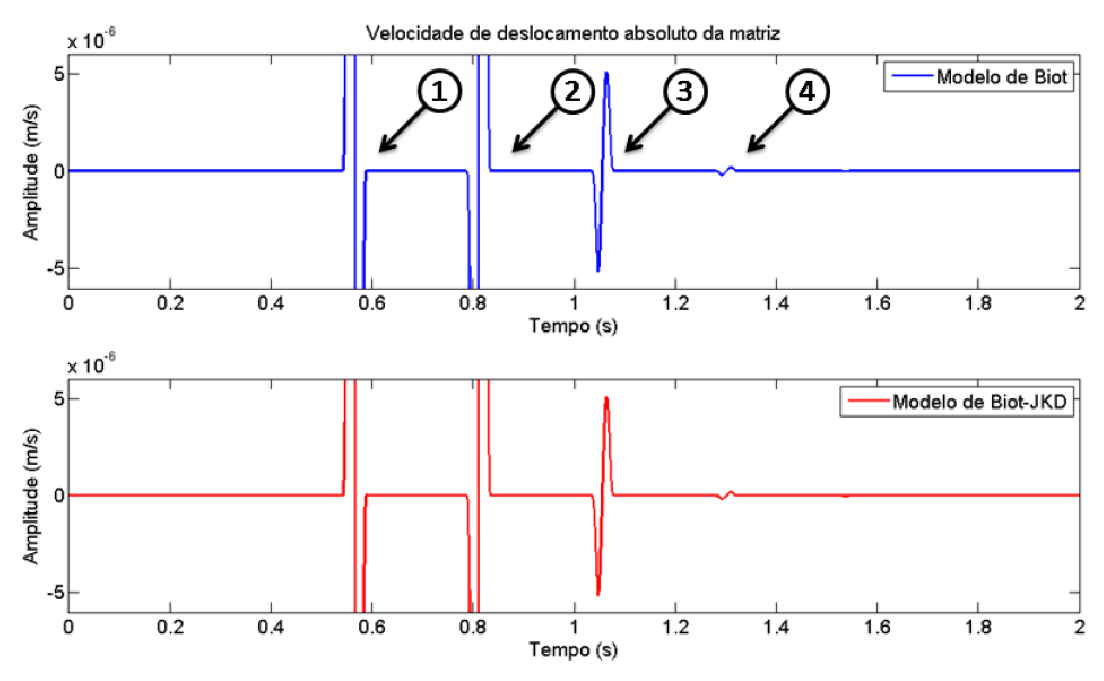
\includegraphics[scale=.65]{igor}
\caption{\textit{Velocidade de deslocamento da matriz para baixas frequ\^encias.}}
\label{fig.igor}
\end{figure}
Al\'em disso, no caso 1D a solu\c{c}\~ao do sistema de Biot pode ser formulada totalmente de maneira anal\'itica e expl\'icita. No caso 3D, todo o c\'odigo computacional s\'o pode ser implementado fazendo uso de opera\c{c}\~oes com matrizes, promovendo desafios em termos de aproxima\c{c}\~oes e instabilidades num\'ericas.


\section{Modelagem Matem\'atica e Num\'erica do Efeito Sismo-Magn\'etico}

Podemos observar uma an\'alise matem\'atica e num\'erica do efeito de indu\c{c}\~ao sismo-magn\'etica em \cite{mikhailenko_97}, onde \'e descrita a solu\c{c}\~ao simult\^anea de equa\c{c}\~oes el\'asticas com o acoplamento da for\c{c}a de Lorentz, e as equa\c{c}\~oes quasi-estacion\'arias de Maxwell com o acoplamento da velocidade de deslocamento do meio de propaga\c{c}\~ao das ondas. Tais sistemas de EDP's foram obtidos do modelo desenvolvido por \cite{Novacki_83} e foram transformadas num sistema de EDO's utilizando transformadas finitas de Fourier.

O sistema de EDO's \'e escrito introduzindo uma matriz de vari\'aveis $A$, e a solu\c{c}\~ao num\'erica \'e obtida pelo m\'etodo de fatoriza\c{c}\~ao encontrado em \cite{Mikhailenko_89}, o qual utiliza a matriz de equa\c{c}\~oes de Riccati para a determina\c{c}\~ao das componentes $a_{ij}$. Tal abordagem n\~ao tem restri\c{c}\~oes computacionais se trabalhada com propaga\c{c}\~ao de ondas de alta frequ\^encia.

As simula\c{c}\~oes foram realizadas considerando ondas longitudinais, transversais e Rayleigh. Os resultados  mostraram, principalmente, que as primeiras chegadas das varia\c{c}\~oes geomagn\'eticas coincidiram com as chegadas dos tipos de ondas que as produziram. Essa coincid\^encia ocorreu para onda longitudinal, Rayleigh e para uma onda refletida na interface entre as camadas.
